% Part: model-theory
% Chapter: interpolation
% Section: separation

\documentclass[../../../include/open-logic-section]{subfiles}

\begin{document}

\olfileid{mod}{int}{sep}

\olsection{\printtoken{P}{sentence} نوں وکھ کرنا}

درمیانی جملے دے قضیے دے ثبوت توں پہلے کجھ
بنیاد رکھنی پئے گی۔ $!A$ تے $!B$ لئی
درمیانی جملہ اوہ !!a{sentence}~$!C$ اے
جس لئی $!A \Entails !C$ تے
$!C \Entails !B$۔ تقابلِ نقیض راہیں
پچھلی گل اوہدوں تے صرف اوہدوں سچ اے جدوں
$\lnot !B \Entails \lnot
!C$۔ ایس خاصیت والے !!^a{sentence}~$!C$
بارے آکھدے آں کہ اوہ \emph{وکھ کردا} اے
$!A$ تے $\lnot !B$ نوں۔ سو $!A$ تے
$!B$ لئی درمیانی جملہ لبھنا، ایسا
!!a{sentence} لبھن دے برابر اے جو $!A$
تے $\lnot !B$ نوں وکھ کرے۔ عام طور وانگ
اک وسیع صورت فائدے والی ہووے گی: ایسا
جملہ جو !!{sentence}s دے دو \emph{سیٹاں}
نوں وکھ کرے۔

\begin{defn}
اک جملہ $!C$، جملیاں دے سیٹاں $\Gamma$
تے $\Delta$ نوں \emph{وکھ کردا} اے اوہدوں
تے صرف اوہدوں جدوں $\Gamma \Entails !C$
تے $\Delta \Entails
\lnot !C$۔ جے ایسا کوئی !!{sentence} موجود
نہ ہووے، تاں $\Gamma$ تے $\Delta$
\emph{وکھ نہ کیتے جا سکّن والے} نیں۔
\end{defn}

$\Gamma$، $\Delta$ تے $!C$ دے نمونیاں
دیاں جماعتاں وچ شمولیت دے تعلق ہیٹھاں
وکھائے گئے نیں:
\begin{figure}[h]
  \centering
  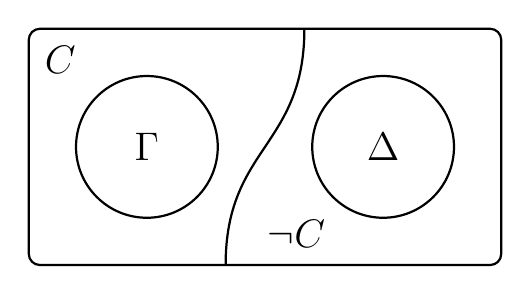
\begin{tikzpicture}[node distance=2cm, auto, thick]
    \draw [rounded corners] (0,0) -- (6,0) -- (6,3) -- (0,3) --  cycle;
    \draw (1.5,1.5) circle (0.9cm);
    \draw (4.5,1.5) circle (0.9cm);
    \path node at (1.5,1.5) {\Large $\Gamma$}; 
    \path node at (4.5,1.5) {\Large $\Delta$}; 
    \path node at (0.4,2.6) {\Large $\formula{C}$};
    \path node at (3.4,0.4) {\Large $\lnot \formula{C}$};
    \draw (2.5,0) .. controls (2.5,1.5) and (3.5,1.5) .. (3.5,3);
  \end{tikzpicture}
  \caption{$!C$، $\Gamma$ تے $\Delta$ نوں وکھ کردا اے}
  \ollabel{fig:sep}
\end{figure}


\begin{lem}\ollabel{lem:sep1}
فرض کرو $\Lang{L}_0$ اوہ زبان اے جس وچ
ہر اوہ !!{constant}، !!{function} تے
!!{predicate} ($\doteq$ توں علاوہ) اے جو
$\Gamma$ تے $\Delta$ \emph{دوہاں}
وچ آؤندا اے؛ تے $\Lang{L}'_0$،
لامتناہی نویں !!{constant}s $\Obj c_n$،
$n \ge 0$ لئی، شامل کرکے ملن والی
زبان ہووے۔ تاں جے $\Gamma$ تے $\Delta$،
$\Lang{L}_0$ وچ وکھ نہ کیتے جا سکّن،
اوہ $\Lang{L}'_0$ وچ وی وکھ نہ کیتے
جا سکّن گے۔
\end{lem}

\begin{proof}
اسیں بالواسطہ ثبوت دیندے آں: تضاد لئی فرض کرو
کہ $\Gamma$ تے $\Delta$،
$\Lang{L}'_0$ وچ وکھ کیتے جا سکدے نیں۔
تاں $\Gamma \Entails
\Subst{!C}{c}{x}$ تے
$\Delta \Entails \lnot \Subst{!C}{c}{x}$
کسے $!C \in \Lang{L}_0$ لئی ہون گے
(ایتھے $c$ اک نواں !!{constant}
اے؛ جے $!C$ وچ ایسے اک توں ودھ نویں
!!{constant} ہون، اوہ صورت وی ایس ورگی اے)۔
محدود گواہی دے قضیے نال \emph{محدود}
ذیلی سیٹ $\Gamma_0$، $\Gamma$ وچوں،
تے $\Delta_0$، $\Delta$ وچوں ملدے نیں،
جنہاں لئی $\Gamma_0 \Entails \Subst{!C}{c}{x}$
تے $\Delta_0 \Entails \lnot \Subst{!C}{c}{x}$۔
$!G$ نوں $\Gamma_0$ دے سارے !!{formula}s
دا منطقی جوڑ، تے $!H$ نوں $\Delta_0$ دے
سارے !!{formula}s دا منطقی جوڑ من لو۔ تاں
\begin{align*}
  !G & \Entails \Subst{!C}{c}{x}, & !H  \Entails \lnot \Subst{!C}{c}{x}.
\end{align*}
پہلے نتیجے توں عمومیت دے قاعدے راہیں
$!G \Entails
\lforall[x][!C]$ ملدا اے؛ دوجے
توں تقابلِ نقیض راہیں
$\Subst{!C}{c}{x} \Entails \lnot !H$
ملدا اے، جس توں
$\lforall[x][!C]
\Entails \lnot !H$ وی۔ فیر
تقابلِ نقیض نال $!H \Entails
\lnot \lforall[x][!C]$ ملدا اے۔
یک رُخیت نال
\begin{align*}
  \Gamma &\Entails \lforall[x][!C], & 
  \Delta & \Entails \lnot \lforall[x][!C],
\end{align*}
ایس لئی $\lforall[x][!C]$،
$\Gamma$ تے $\Delta$ نوں
$\Lang{L}_0$ وچ وکھ کردا اے۔
\end{proof}

\begin{lem}\ollabel{lem:sep2}
فرض کرو $\Gamma \cup \{ \lexists[x][!S] \}$
تے $\Delta$ وکھ نہ کیتے جا سکّن، تے
$c$ اک نواں !!{constant} ہووے جو
$\Gamma$، $\Delta$ یا $!S$ وچ نہ ہووے۔
تاں $\Gamma \cup \{ \lexists[x][!S], \Subst{!S}{c}{x} \}$
تے $\Delta$ وی وکھ نہ کیتے جا سکّن گے۔
\end{lem}

\begin{proof}
تضاد لئی فرض کرو کہ $!C$،
$\Gamma \cup \{
\lexists[x][!S], \Subst{!S}{c}{x}\}$
تے $\Delta$ نوں وکھ کردا اے، جدوں کہ
نال ہی $\Gamma \cup \{\lexists[x]{!S} \}$
تے $\Delta$ وکھ نہ کیتے جا سکدے ہون۔
دو صورتاں وکھ کردے آں:
\begin{enumerate}
\item جے $c$، $!C$ وچ نہ آوے، تاں
  $\Gamma \cup
  \{\lexists[x][!S], \lnot!C \}$
  پورا ہون جوگا اے (ورنہ $!C$،
  $\Gamma \cup \{\lexists[x][!S] \}$
  تے $\Delta$ نوں وکھ کردا)۔
  $\Subst{!S}{c}{x}$ شامل کرن توں بعد وی
  ایہ پورا ہون جوگا رہندا اے؛ ایس لئی
  $!C$، $\Gamma \cup \{ \lexists[x][!S], \Subst{!S}{c}{x} \}$
  تے $\Delta$ نوں آخرکار وکھ نہیں کردا۔
\item جے $c$، $!C$ وچ آوے، تاں
  $!C$ دی صورت
  $\Subst{!C}{c}{x}$ اے۔ ایس توں
  \[
  \Gamma \cup \{ \lexists[x][!S], \Subst{!S}{c}{x}\} \Entails \Subst{!C}{c}{x},
  \]
  ملدا اے؛ فیر استنباط دے قضیے
  تے عمومیت نال
  $\Gamma, \lexists[x][!S] \Entails \lforall[x][(!S \lif !C)]$
  تے آخر $\Gamma
  \cup \{ \lexists[x][!S] \} \Entails \lexists[x][!C]$۔
  دوجے پاسے $\Delta \Entails \lnot \Subst{!C}{c}{x}$
  اے؛ سو عمومیت نال
  $\Delta \Entails \lnot \lexists[x][!C]$۔
  ایس لئی $\Gamma
  \cup \{\lexists[x][!S] \}$
  تے $\Delta$ وکھ کیتے جا سکدے نیں،
  جو تضاد اے۔
\end{enumerate}
\end{proof}

\end{document}
